\section{Implementierung}
Im nachfolgenden Kapitel wird beschrieben, welche Technologien eingesetzt wurden und wie die Architektur der Anwendung aussieht. Des weiteren werden die wichtigsten AngularJS Services und Direktiven vorgestellt, die für die Anwendung implementiert wurden und es wird beschrieben, wie die Benutzeroberflächen umgesetzt worden sind.

 \subsection{Verwendung von AngularJS für alle Komponenten des Plugins}
 Für die Implementierung von Jarvis wurde sich für AngularJS\footnote{\url{https://angularjs.org/}} entschieden. Das von Google entwickelte JavaScript MVC-Framework bietet einige Vorteile, die Webentwicklung im Allgemeinen und die Entwicklung dieser Extension erleichtern.

 AngularJS erlaubt es eigene Direktiven zu entwerfen. Direktiven beschreiben wie ein HTML Element dargestellt werden soll und wie es (z.B. auf Benutzerinteraktionen) reagieren soll \cite{jain2015angularjs}. Sie können dann wie HTML Tags oder Attribute genutzt werden. So wird eine hohe Wiederverwendbarkeit von Komponenten erzeugt. Genutzt wurde dieses Feature um eine Direktive zu entwickeln, mit der die Paragraphen der Webseite ``verpackt'' werden. Die neue Direktive enthält die Funktionen um eine Suchanfrage zu bauen und zu senden und die graphischen Elemente um die Resultate anzuzeigen. 

 Weiterhin befindet sich in den meisten Frameworks das Markup in einem Template. Dieses Template wird dann in HTML Code kompiliert und in das Document Object Model (DOM) geladen \cite{jain2015angularjs}. Das Markup der AngularJS Application befindet sich innerhalb des HTML-Dokuments. Dadurch ist es möglich, dass AngularJS das Markup erst auswertet, nachdem es in das DOM geladen wurde \cite{jain2015angularjs}. Von den Vorteilen die dadurch entstehen ist einer für die Entwicklung von Jarvis besonders nützlich: Da AngularJS die Seite erst nach dem Laden auswertet, ist es einfach, AngularJS Module in existierende Webseiten zu integrieren \cite{jain2015angularjs}. Mit Jarvis möchte genau das erreicht werden. Zu einer bestehenden Seite soll Funktionalität hinzugefügt werden. Zusammen mit JavaScript Injection kann man auf diese Weise innerhalb des Client-Browsers AngularJS Logik in eine beliebige Seite integrieren, ohne die eigentliche Implementierung der Seite zu verändern.

 Der Modul-basierte Aufbau von AngularJS Anwendungen gestattet außerdem eine leichte Erweiterbarkeit und Austauschbarkeit der Komponenten. Einzelne Dienste, wie bei Jarvis die Extrahierung der Schlüsselwörter oder die Kommunikation mit Europeana, sind in Module oder Services verpackt und können so einfach durch andere ersetzt werden. So kann man die Extension leicht auf andere Suchmaschinen umbauen oder andere Algorithmen zur Analyse der Paragraphen verwenden.

 Unabhängig von der Entwicklung von Jarvis bietet AngularJS einen weiteren großen Vorteil: Two way data-binding \cite{jain2015angularjs}. Im Gegensatz zu anderen Frameworks oder zu reinem JavaScript, wo man manuell jede Änderung des Models an die View propagieren muss und anderes herum, übernimmt AngularJS diese Aufgabe. Ändert sich das Model, wird automatisch das jeweilige DOM Element angepasst. Interagiert der User mit einem Element, werden Änderungen sofort an das dahinter stehende Model weitergeben. Das reduziert den benötigten Code und erlaubt eine schnelle und saubere Entwicklung von Anwendungen.

 \subsection{Architektur der Extension}
 Wie in Abbildung \ref{fig:architektur} zu sehen ist, ist Jarvis in vier AngularJS Module unterteilt:
 \begin{enumerate*}[label=\alph*\upshape)]
 	\item Jarvis für die Content-Skripte,
  	\item JarvisBG für die Background-Skripte,
 	\item JarvisPopup für die Browser-Action, und
 	\item JarvisSettings für die Options-Page.
 \end{enumerate*}
 Im folgenden Absatz beschreibt Jarvis das Modul der Content-Skripte und nicht die gesamte Extension.

 \begin{minipage}{\linewidth}
	\centering
	\vspace*{0.5cm}
	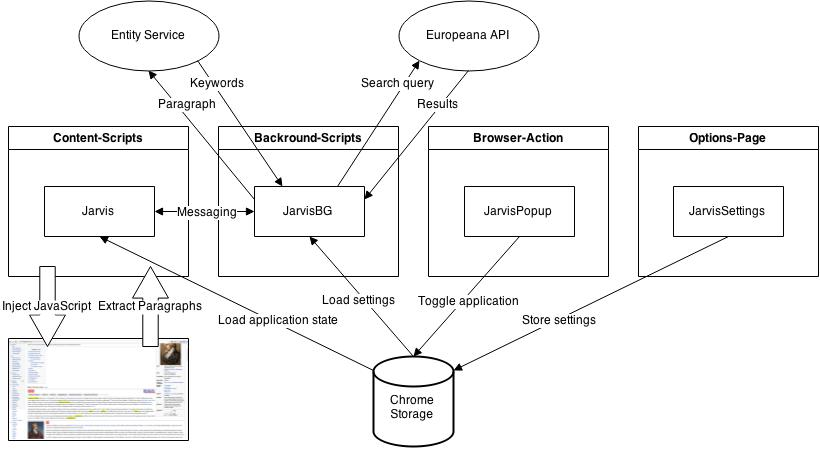
\includegraphics[width=\linewidth]{Bilder/architektur.jpg}
	\captionof{figure}{Kommunikation der AngularJS Komponenten untereinander}
	\label{fig:architektur}
	\vspace*{0.5cm}
 \end{minipage}
 
 Jarvis ist das Modul, welches in die jeweilige Webseite per JavaScript Injection eingefügt wird. Es extrahiert die Paragraphen aus dem Text und fügt die eigene Direktive (im Folgenden Paragraph-Directive genannt) in das DOM ein. Die extrahierten Paragraphen werden per Message Passing\footnote{\url{https://developer.chrome.com/extensions/messaging}} an die Background-Skripte weitergegeben. Diese sind zusammengefasst im Modul JarvisBG. 

 Dieses Modul ist zuständig für die Kommunikation mit den REST Endpunkten von Europeana und dem Entity Service. Im Gegensatz zu Jarvis, welches für jeden offenen Browser-Tab eine eigene Instanz hat, existiert das JarvisBG Modul nur ein mal (wie auch JarvisPopup und JarvisSettings). Jarvis schickt Nachrichten mit dem Namen des angeforderten Services sowie einer Callback-Methode an JarvisBG. Dieses führt die Anfrage aus und übergibt die Ergebnisse der Callback-Methode. Diese sorgt dann dafür, dass die Ergebnisse im Frontend richtig angezeigt werden. 

 JarvisPopup ist das Modul des Popup-Fensters, welches nach klick auf das Icon der Extension rechts des Adressfeldes angezeigt wird. Über das Popup wird der Zustand der Extension im aktuellen Tab gesteuert. Der User kann hier entscheiden, ob das Programm in diesem Tab angezeigt wird oder nicht. Der Zustand wird dann im Chrome Storage\footnote{\url{https://developer.chrome.com/extensions/storage}} gespeichert. Die Wahl für die Speicherung der Anwendungsdaten viel auf den Chrome Storage, da er einige Vorteile gegenüber der localStorage API\footnote{\url{https://developer.mozilla.org/en-US/docs/Web/Guide/API/DOM/Storage\#localStorage}} bietet. Zum einen können die Content-Skripte direkt darauf zugreifen ohne einen Umweg über die Background-Skripte gehen zu müssen. Weiterhin erlaubt Chrome Storage eine automatische Synchronisierung der Inhalte. Dadurch wird Jarvis sofort benachrichtigt, sobald sich der Zustand der Applikation ändert.

 Der Nutzer hat die Möglichkeit, über die Options-Page\footnote{\url{https://developer.chrome.com/extensions/optionsV2}} die verwendeten Services zu konfigurieren. Das dafür zuständige Modul ist JarvisSettings. Es speichert die Einstellungen im Chrome Storage und JarvisBG passt die REST-Anfragen entsprechend an.

 \subsection{Eigene Services und Direktiven}
 Um eine Hohe Modularität und Austauschbarkeit zu gewährleisten sowie eine übersichtliche Architektur zu schaffen wurden einzelne Funktionalitäten in AngularJS Services und Direktiven ausgelagert. So können zum Beispiel die Services zur Kommunikation mit Europeana oder zum Finden der Schlüsselwörter einfach ausgetauscht werden um andere Algorithmen/Informations-Quellen zu benutzen. Die wichtigsten Services und Direktiven werden hier vorgestellt.

  \subsubsection{ParagraphDetectionService}
  Jarvis teilt die aktuelle Webseite in Paragraphen ein. In diesem Fall sind damit nicht HTML Paragraphen Tags gemeint, sondern jegliche zusammenhängende Textpassage die größer als ein bestimmter Schwellwert ist. Der Algorithmus dafür stammt vom Lehrstuhl für Medieninformatik an der Universität Passau.
 
  Um Paragraphen innerhalb der Seite zu finden wird das DOM mit einem TreeWalker\footnote{\url{http://www.javascriptkit.com/dhtmltutors/treewalker.shtml}} durchlaufen. Es werden alle Knoten herausgefiltert, deren Vorgängerknoten Script, Style oder Noscript Tags sind, sowie Knoten die keinen Text oder weniger als 40 Zeichen enthalten. Die restlichen Knoten werden nun einzeln betrachtet um zusammenhängende Paragraphen zu erkennen. Dazu werden jeweils die Nachbarknoten betrachtet. Gibt es einen Nachbarknoten der kein reiner Textknoten ist und sich ebenfalls in der Liste der gefundenen Paragraphen befindet so werden beide als zusammengehörig abgespeichert. Alle Knoten zu denen kein passender Nachbar gefunden wurde, die jedoch mehr als 100 Zeichen haben und mindestens einen ``.'', werden als einzelne Paragraphen gespeichert.

  Daraufhin werden nochmal alle zusammengehörigen und einzelnen Paragraphen durchlaufen. Dabei wird der Vorgängerknoten jedes Elements betrachtet. Ist dieser ein Header Knoten so wird er als Überschrift des Paragraphen gespeichert. Jedes Element wird dann in die ParagraphDirective eingebettet.

  Schlussendlich werden noch alle Anchor Tags innerhalb der Paragraphen entfernt. Sie verhindern das Auswählen eines Schlüsselwortes aus dem Text per Doppelklick und werden deshalb durch AnchorDirectives ersetzt. 

  Verpackt ist dieser Algorithmus in einen AngularJS Service (ParagraphDetectionService), der im Modul Jarvis registriert ist. Nach dem Laden der Extension führt er die Paragraphen-Suche aus und stellt Funktionen zum abrufen der gefunden Textpassagen bereit.
 
  \subsubsection{KeywordService}
  Um aus den gefundenen Paragraphen die wichtigen Schlüsselwörter zu extrahieren wird ein REST-Service genutzt (im Konzept Entity Service genannt), der auch vom Lehrstuhl für Medieninformatik an der Universität Passau bereitgestellt wurde. Dieser Service basiert auf DBpedia Spotlight\footnote{\url{http://spotlight.dbpedia.org/}}, einem System zum automatischen Annotieren von DBpedia\footnote{\url{http://wiki.dbpedia.org/}} Entities in Texten \cite{daiber2013improving}. 

  DBpedia Spotlight ist ein Open Source Projekt, das einen REST-Service entwickelt hat, welcher Interfaces für Phrase Spotting (Erkennen von Ausdrücken, die annotiert werden können) und Disambiguierung (Assoziieren von Phrasen mit DBpedia Entities) anbietet \cite{daiber2013improving}. Dabei analysiert der Service einen Text in vier Phasen:

  Während des Phrase Spottings werden die Phrasen innerhalb des Textes gesucht, die zu einer DBpedia Ressource passen könnten. Dazu durchläuft ein String-Matching-Algorithmus den Text. Als Suchmaske wird ein Set aus Labels genutzt, welches aus DBpedia Ressourcen gewonnen wurde \cite{mendes2011dbpedia}. Danach folgt die Candidate Selection: Den gefundenen Kandidaten werden mögliche Disambiguierungen aus dem DBpedia Lexikalisierungs Datensatz zugewiesen. Im nächsten Schritt, der Disambiguation, wird der Kontext - der ursprüngliche Text - dazu genutzt die am besten passenden Disambiguierungen für jeden Kandidaten zu finden. Dazu wird aus den DPpedia Ressourcen ein Vektor Space Model gewonnen und die möglichen Disambiguierungen werden nach der Ähnlichkeit ihres Kontext-Vektors und dem Kontext des Ursprungstextes bewertet. Der letzte Schritt bietet dem User die Möglichkeit den Prozess zu personalisieren. Er kann zum Beispiel Listen mit erlaubten oder verbotenen Entities übergeben, die in der Candidate Selection genutzt werden \cite{mendes2011dbpedia}. Zum Schluss werden die finalen Kandidaten und die jeweils passende Disambiguierung zurück gegeben. 

  Die erhaltenen Kandidaten werden dann als Schlüsselwörter für die Suche bei Europeana genutzt. Allerdings sind diese Kandidaten nicht immer Wörter oder Phrasen, die direkt im Text vorkommen. So wird zum Beispiel das Wort ``Marbach'' nicht genauso wieder zurück gesendet, sondern der dazugehörige Kandidat wäre ``Marbach am Neckar''. So wird zwar eine höhere Genauigkeit erzielt, jedoch können diese Kandidaten dann nicht wie die anderen Schlüsselwörter der Suche im Paragraphen hervorgehoben werden (siehe Kapitel \ref{ssec:suchanfragenGenerierung}).
 
  Aufgerufen wird der Entity Service aus einem AngularJS Service (KeywordService), welcher den erhaltenen Entities noch einen Score zu weißt. Der Score errechnet sich aus der Anzahl der Vorkommen der Entity im Paragraphen und einer Gewichtung der Entity-Typen. Ist der Score größer als ein gegebener Schwellwert, wird die Entity in die Ergebnisliste eingefügt. Der KeywordService, welcher im JarvisBG Modul registriert ist, gibt darauf hin die Liste mit den Ergebnissen zurück.

  \subsubsection{MessageService}
  Es gibt zwei Versionen des MessageServices. Eine ist im Jarvis Modul registriert und eine im JarvisBG Modul. Die Aufgabe des MessageService, welcher Teil von Jarvis ist, ist die Weiterleitung von Nachrichten aus den Content-Skripten an die Background-Skripte. Dazu wird das Message Passing der Chrome API verwendet. Eine Nachricht besteht dabei aus drei Teilen:
  \begin{enumerate*}
 	\item Die ID der Extension, deren Background-Skripte angesprochen werden sollen,
  	\item der Name des gewünschten Services und der Methode die in ihm aufgerufen werden soll sowie
 	\item eine Callback-Methode die vom Empfänger nach der Abarbeitung der Nachricht aufgerufen werden soll. 
  \end{enumerate*} 

  Der MessageService im JarvisBG Modul hört auf Nachrichten die an die Background-Skripte gesendet werden. Hier werden alle zur Verfügung stehenden Services registriert. Kommt eine Nachricht an, extrahiert der er den Namen des gewünschten Services sowie den Namen der Methode und führt diese aus. Die Ergebnisse, die von der ausgeführten Methode zurückgeliefert wurden, übergibt er dann der Callback-Methode. Weiterhin stellt er Funktionen zur Kommunikation mit den Content-Skripten in den verschiedenen Browser Tabs bereit.

  \subsubsection{ParagraphDirective}
  Die ParagraphDirective umschließt die Paragraphen der Seite. Sie beinhaltet die GUI Elemente zur Manipulation der Schlüsselwörter sowie zur Anzeige der Ergebnisse. 

  Der Controller der Direktive synchronisiert sich mit dem Chrome Storage um auf Zustandsänderungen der Extension zu reagieren. Deaktiviert der User die Anwendung über das Popup, werden die graphischen Elemente der ParagraphDirective ausgeblendet. Wird sie aktiviert erscheinen sie wieder. Klickt der User auf den Suchbutton, wird eine Anfrage, die den Text des jeweiligen Paragraphen beinhaltet, an JarvisBG gesendet. Dazu wird der schon erwähnte MessageService genutzt. Sobald die Ergebnisse vom KeywordService in der Direktive ankommen, wird eine Suchanfrage mit den gefundenen Schlüsselwörtern über die Background-Skripte an Europeana gesendet. Icons zum Ansehen der Quellen werden bei Ankunft der Ergebnisse neben den gefundenen Schlüsselwörtern angezeigt.

  \subsubsection{AnchorDirective}
  Der User soll per Doppelklick Wörter im Text auswählen können und sie so zur Suchanfrage hinzufügen können. Auch das Löschen von Schlagwörtern durch Doppelklick auf hervorgehobene Wörter im Text soll möglich sein. Ein Problem dabei sind Hyperlinks. Bei einem Klick auf einen Anchor Knoten wird sofort der zugewiesene Link aufgerufen. Ein Doppelklick funktioniert also nicht da die neue Seite schon geladen wurde. Um dieses Problem zu umgehen wurde eine neue Direktive entworfen, die das Verhalten von Anchor Tags imitieren soll. Sie übernimmt alle Eigenschaften wie Titel und CSS Klassen vom ursprünglichen Anchor Tag. Die Zieladresse des Hyperlinks wird der neuen AnchorDirektive übergeben und dort gespeichert. Bei einem Klick auf die Direktive wird ein Countdown von 300 ms gestartet. Wird während dieser Zeit kein zweiter Klick registriert lädt die Direktive die Seite des Hyperlinks. Macht der User jedoch einen Doppelklick, verhindert sie, dass sich die Seite ändert.

 \subsection{Implementierung der GUIs}
 In diesem Teil wird beschrieben wie das Konzept des Ramping Interfaces umgesetzt wurde und wie man versucht hat zu Erreichen, dass die zusätzlichen Elemente die Aufmerksamkeit des Users nicht zu sehr belasten. Für die Beschreibung der GUI Elemente wird ``Hover'' als Beschreibung für den Zustand eines Elements eingeführt, auf welchem sich gerade der Cursor der Maus befindet. Als Farbpalette für die Extension wurde sich für blau und rot entschieden, da sich diese Farben von den meisten Designs gut abheben. So erkennt der Nutzer leicht, welche Elemente zur Extension gehören und welche zur ursprünglichen Webseite. 
 
 \begin{minipage}{\linewidth}
	\centering
	\vspace*{0.5cm}
	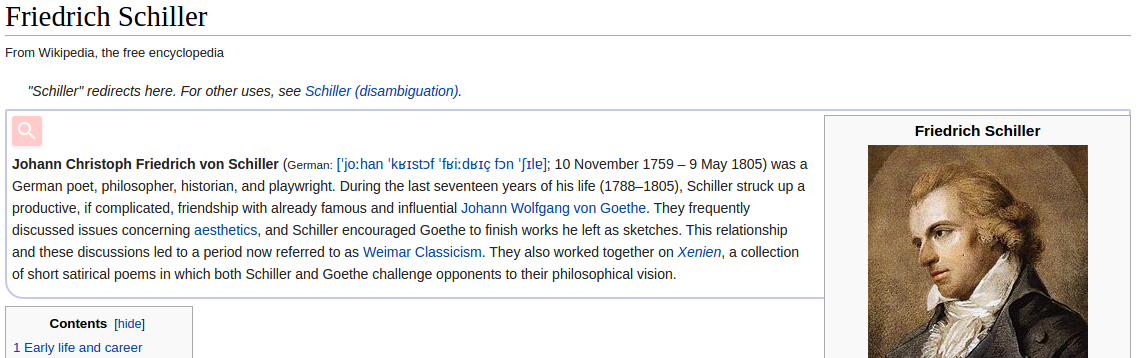
\includegraphics[width=\linewidth]{Bilder/app-screenshots/paragraph-unhovered.png}
	\captionof{figure}{Hervorgehobener Paragraph}
	\label{fig:paragraph}
	\vspace*{0.5cm}
 \end{minipage}

 Ist die Extension aktiviert und geladen, werden alle gefundenen Paragraphen mit einem Rahmen umschlossen (siehe Abbildung \ref{fig:paragraph}). So wird verdeutlicht, was alles zu einem Abschnitt dazugehört. Im oberen linken Eck des Paragraphen befindet sich ein Icon mit dem zuerst die Analyse des Paragraphen-Inhalts gestartet wird und anschließend automatisch eine Anfrage an Europeana gesendet wird.

 \begin{minipage}{\linewidth}
	\centering
	\vspace*{0.5cm}
	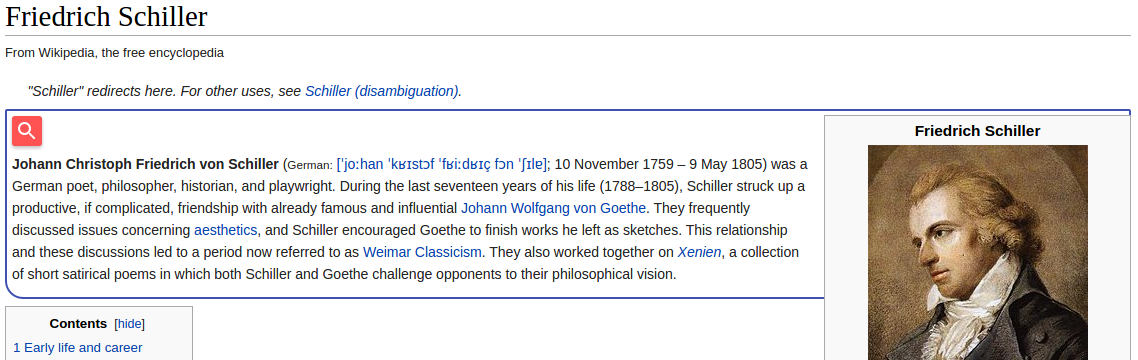
\includegraphics[width=\linewidth]{Bilder/app-screenshots/paragraph-hovered.png}
	\captionof{figure}{Hervorgehobener Paragraph im Hover-Zustand}
	\label{fig:paragraphHover}
	\vspace*{0.5cm}
 \end{minipage}

 Um den Nutzer nicht unnötig abzulenken, verlieren die Elemente der einzelnen ParagraphDirectives an Deckkraft, wenn sie nicht im Hover Zustand sind, also der Cursor sich nicht über dem Element befindet. Fährt der User mit der Maus über einen Paragraphen, erscheint er wieder in voller Farbe (siehe Abbildungen \ref{fig:paragraph} und \ref{fig:paragraphHover}).

 \begin{minipage}{\linewidth}
	\centering
	\vspace*{0.5cm}
	\includegraphics[width=\linewidth]{Bilder/app-screenshots/keywords.png}
	\captionof{figure}{Anzeige der gefundenen Keywords sowie Anzahl der Ergebnisse}
	\label{fig:keywords}
	\vspace*{0.5cm}
 \end{minipage}

 Sobald Schlüsselwörter zur Verfügung stehen, werden sie im Text hervorgehoben sowie oberhalb des Textes angezeigt (siehe Abbildung \ref{fig:keywords}). Dieser Fall tritt ein, wenn der Nutzer per Doppelklick ein Wort im Text ausgewählt hat oder wenn er durch Betätigen des Knopfes die Analyse des Paragraphen ausgelöst hat. Zur Anzeige der Schlüsselwörter wurden md-chips\footnote{\url{https://material.angularjs.org/latest/\#/api/material.components.chips/directive/mdChips}} verwendet. Diese Direktive aus der Angular Material Bibliothek gestattet die einfache Darstellung von Listenelementen und bietet zudem intuitive Steuerungsmöglichkeiten. Durch einen Klick auf das Kreuz neben einem Schlüsselwort kann dieses entfernt werden. Zudem kann mit den Pfeiltasten zwischen den Schlüsselwörtern hin und her gewechselt werden und durch das Betätigen der Entfernen-Taste kann das ausgewählte Element entfernt werden. Die md-chips Direktive bietet zudem eine gute Möglichkeit für die Zukunft, um Relevance Feedback umzusetzen. Darauf wird in Kapitel \ref{sec:futureWork} genauer eingegangen.

 Sobald Ergebnisse von Europeana zur Verfügung stehen, erscheinen im oberen rechten Eck des Paragraphen drei Icons, eines für jeden Quellen-Typ. Ein Zähler an jedem Icon signalisiert dem User, wie viele Ergebnisse zum jeweiligen Quellen-Typ gefunden wurden. Nach einem Klick auf eines der Icons öffnet sich ein Dialog mit den Ergebnissen.

 Hat der User die Schlüsselwörter angepasst, kann er mit einem Klick auf das neu erschienene Icon neben dem Suchsymbol eine erneute Suchanfrage an Europeana schicken, ohne den Paragraphen nochmals nach Schlüsselwörtern durchsuchen zu lassen.

 \begin{minipage}{\linewidth}
	\centering
	\vspace*{0.5cm}
	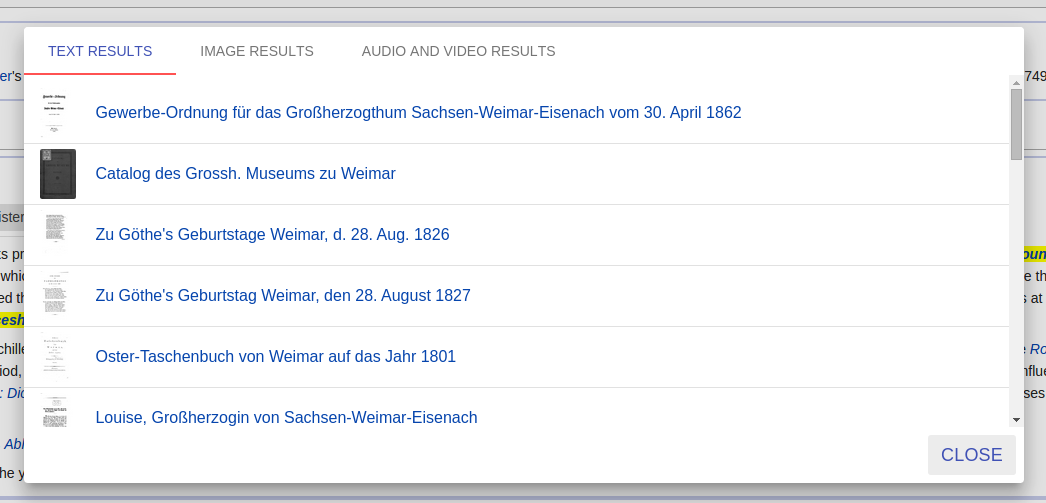
\includegraphics[width=\linewidth]{Bilder/app-screenshots/text-results.png}
	\captionof{figure}{Dialog mit gefundenen Textquellen}
	\label{fig:textResults}
	\vspace*{0.5cm}
 \end{minipage}

 Abbildung \ref{fig:textResults} zeigt den Dialog für textuelle Ergebnisse. Mit dem oberen Reiter kann der User zwischen den Quellen-Typen umschalten. Text-Quellen sowie Audio- und Video-Quellen werden in einer Liste dargestellt. Die Listenelemente bestehen aus einem Miniaturbild und dem Titel der Quelle. Durch einen Klick auf das Bild oder den Titel gelangt der der User direkt zu Europeana, wo sich die Ressource befindet. Fährt er mit der Maus über das Miniaturbild wechselt das Element in den Hover-Zustand. 

 \begin{minipage}{\linewidth}
	\centering
	\vspace*{0.5cm}
	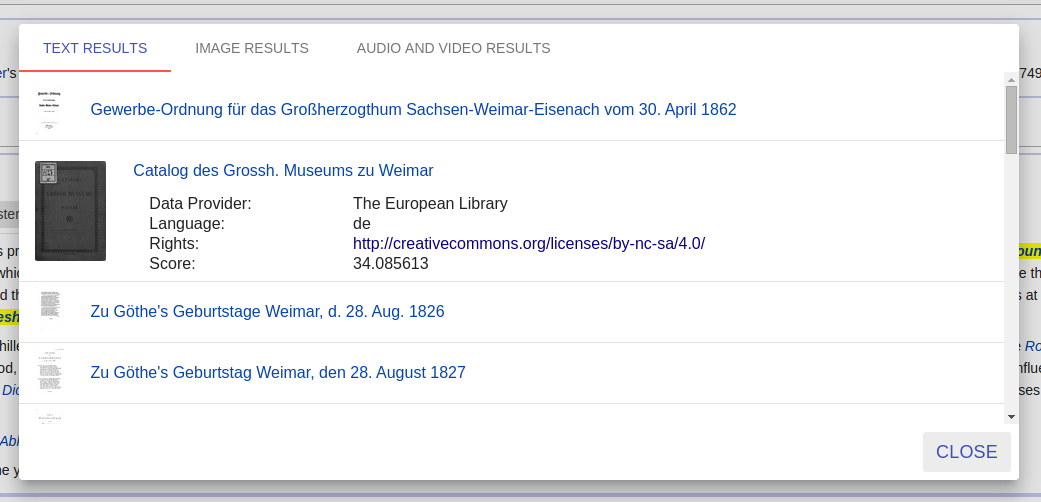
\includegraphics[width=\linewidth]{Bilder/app-screenshots/text-results-hovered.png}
	\captionof{figure}{Detaillierte Ansicht einer Textquelle}
	\label{fig:textResultsHover}
	\vspace*{0.5cm}
 \end{minipage}

 Der Hover-Zustand ist gleichzeitig die letzte Stufe des Ramping Interfaces. Nach der Anzahl der gefundenen Quellen und Miniaturbild und Titel der Quellen werden nun detailliertere Informationen angezeigt. Wie in Abbildung \ref{fig:textResultsHover} zu sehen ist wird jetzt das Bild der Quelle vergrößert. Außerdem werden unter dem Titel noch der Anbieter der Ressource sowie Sprache und Nutzungsrechte dargestellt. Die Ergebnisse sind nach einem Relevance Score sortiert, den die Europeana API für jede Quellen mitsendet. Je höher der Score umso höher die Wahrscheinlichkeit, dass die Ressource für den User interessant ist. Dieser Wert wird ebenfalls angezeigt. 

 \begin{minipage}{\linewidth}
	\centering
	\vspace*{0.5cm}
	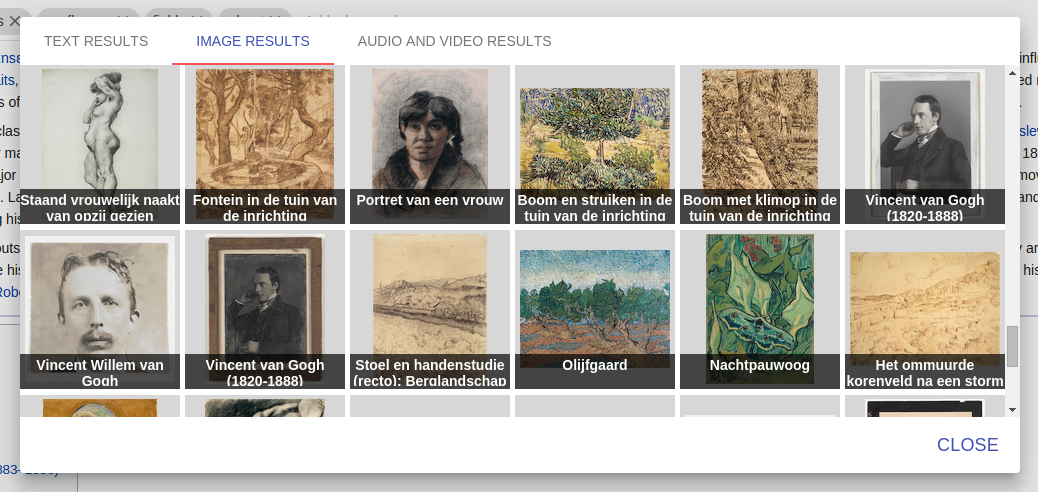
\includegraphics[width=\linewidth]{Bilder/app-screenshots/image-results.png}
	\captionof{figure}{Dialog mit gefundenen Bildquellen}
	\label{fig:imageResults}
	\vspace*{0.5cm}
 \end{minipage}

 Bei Bildquellen sind Metadaten wie die Sprache der Ressource nicht so Relevant wie das eigentliche Bild. Aus diesem Grund wurde für die Anzeige der Bildquellen eine andere Darstellungsweise gewählt. Die Ergebnisse werden in einer md-grid-list\footnote{\url{https://material.angularjs.org/latest/\#/api/material.components.gridList/directive/mdGridList}} angezeigt. Die Elemente der Liste bestehen aus dem Bild sowie dem Titel. Auch hier gelangt der User durch einen Klick direkt zur Ressource, jedoch existiert kein separater Hover-Zustand.

 Ist ein Vorschaubild nicht verfügbar oder wurden keine Quellen des ausgewählten Typs gefunden, wird stattdessen ein Platzhalter an der entsprechenden Stelle angezeigt.

 \begin{minipage}{\linewidth}
	\centering
	\vspace*{0.5cm}
	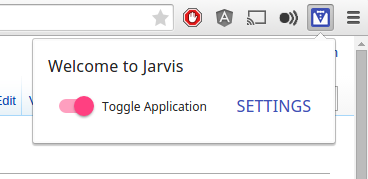
\includegraphics[scale=0.6]{Bilder/app-screenshots/popup.png}
	\captionof{figure}{Popup zum aktivieren der Extension}
	\label{fig:popup}
	\vspace*{0.5cm}
 \end{minipage}

 Um die Extension zu aktivieren oder deaktivieren muss der User auf das Jarvis-Icon neben der Adressleiste des Browsers klicken. Dadurch öffnet sich ein Popup (siehe Abbildung \ref{fig:popup}). Durch einen Klick auf den Umschalter wechselt die Anwendung ihren Zustand. Allerdings gilt dies nur für den aktuellen Tab. Die Jarvis Module in anderen Tabs sind dadurch nicht betroffen. Weiterhin bietet das Popup dem User einen Knopf an, mit dem er zum Einstellungsdialog gelangt.

 \begin{minipage}{\linewidth}
	\centering
	\vspace*{0.5cm}
	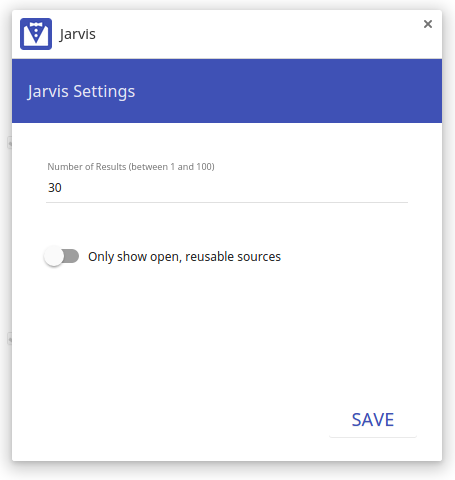
\includegraphics[scale=0.5]{Bilder/app-screenshots/settings.png}
	\captionof{figure}{Dialog zum anpassen der Einstellungen}
	\label{fig:settings}
	\vspace*{0.5cm}
 \end{minipage}

 Die Einstellungen der Extension können über ein separates Fenster angepasst werden. Der in Abbildung \ref{fig:settings} dargestellte Dialog ist über den Extension Manager\footnote{Innerhalb von Chrome zu finden unter: \url{chrome://extensions/}}, sowie über den erwähnten Knopf im Popup, erreichbar. Er bietet momentan die Möglichkeit die Anzahl der Ergebnisse fest zu legen, die von Europeana geliefert werden sollen. Auch kann der User entscheiden ob er alle Quellen sehen möchte, oder nur solche, die er weiterverwenden und bearbeiten darf.